\begin{figure}[htbp]
    \centering
    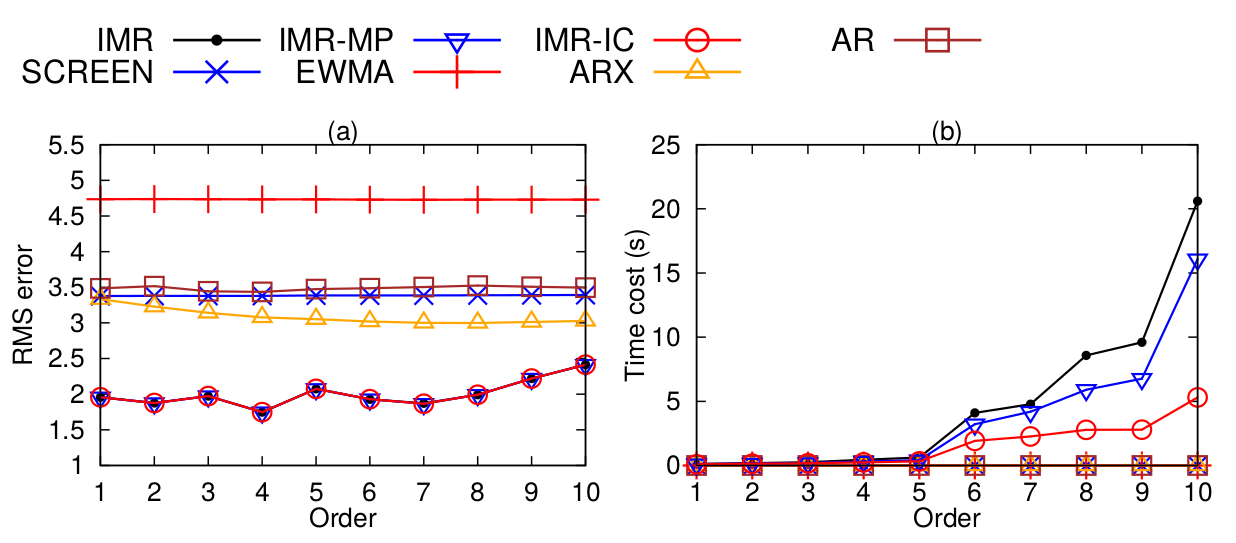
\includegraphics[width=\textwidth]{../plots/varying_order_p.png}
    \caption{Unterschiedliche Ordnung $p$ über GPS-Daten mit $\tau$ = 0.2, Datengröße 750 und Markierungsrate 0.2}%
    \label{varying_order_p}
\end{figure}
\begin{figure}[htbp]
    \centering
    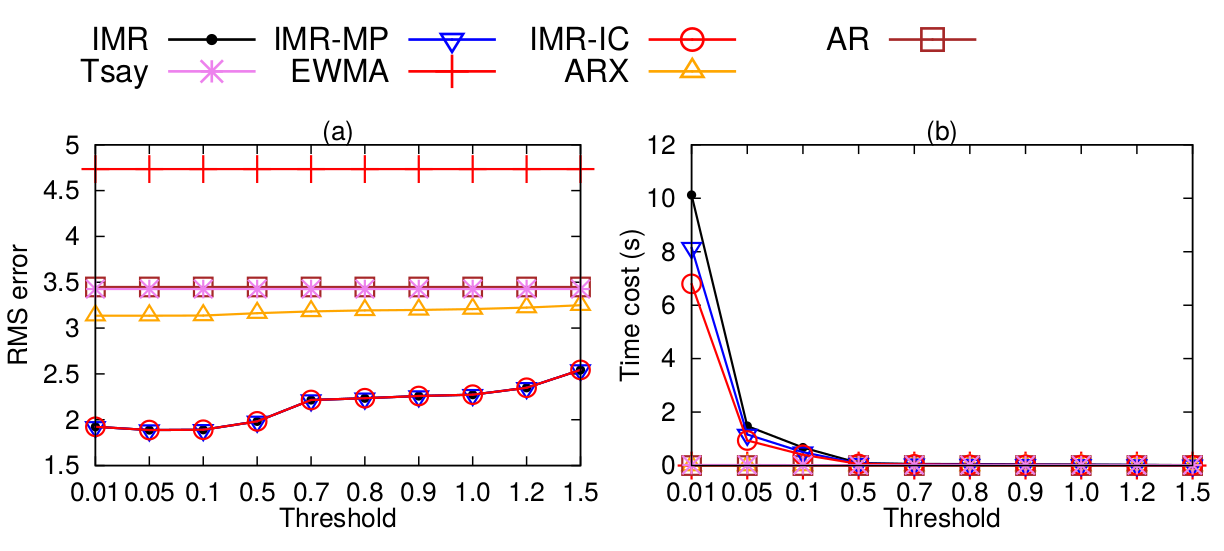
\includegraphics[width=\textwidth]{../plots/varying_threshold.png}
    \caption{Unterschiedliche Schwellenwerte $\tau$ über GPS-Daten mit $p$ = 3, Datengröße 750 und Markierungsrate 0.2}%
    \label{varying_threshold}
\end{figure}
\begin{figure}[htbp]
    \centering
    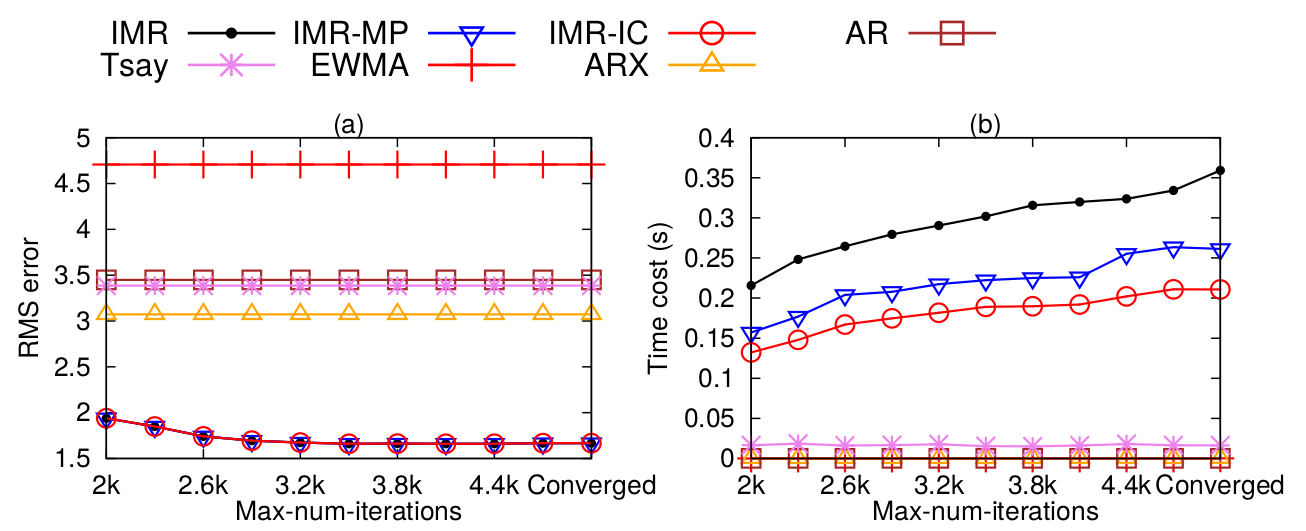
\includegraphics[width=\textwidth]{../plots/varying_maximum_number.png}
    \caption{Unterschiedliche maximale Anzahl von Iterationen über GPS-Daten mit $\tau = 0,2$, $p$ = 3 und Datengröße 750}
    \label{varying_maximum_number}
\end{figure}
\begin{figure}[htbp]
    \centering
    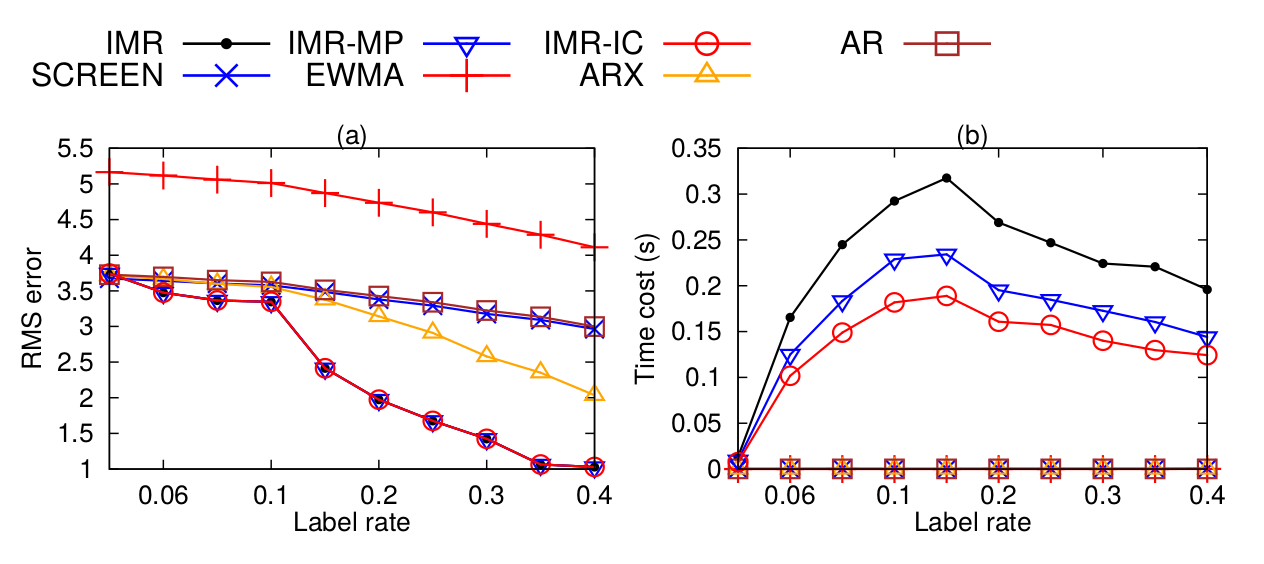
\includegraphics[width=\textwidth]{../plots/varying_labeling_rate.png}
    \caption{Unterschiedliche Markierungsraten über GPS-Daten mit $\tau = 0,2$, $p$ = 3 und Datengröße 750}
    \label{varying_labeling_rate}
\end{figure}
